\chapter{Digital filter}

\section{Design}

The goal of this lab is to digitally filter a waveform sampled at 44.1kHz and downsample it to a frequency of $F_{sampling}=22.05$ kHz. To perform this subsampling, it is necessary that the signal is composed of frequencies smaller than the Nyquist frequency : 
\[ F \le F_N = \frac{F_{sampling}}{2} \] 
Thus, all frequencies higher than $ F_N = 11.025$ kHz have to be filtered out by a low pass filter.\\
\\
As it is known, an ideal low pass filter is defined by its impulse response: 
\[ h(n) = B*sinc(Bn) = B * \frac{sin(\pi Bn)}{\pi Bn} \] where \[B = 2*f_{cutoff}\]
This filter is however neither causal nor finite, and therefore not feasible. To overcome this problem, it is necessary to find a window $w(n)$, such that $h(n)*w(n)$ is finite and causal. In our case, the choice is made to use the rectangle window, for reasons of simplicity : \[ w(n) = \left\{
\begin{array}{ll}
1 & \mbox{if } \vert n \vert  \le N\\
0 & \mbox{otherwise}
\end{array}
\right. \]
where $N$ is the filter order. It is noteworthy that the order $N$ must be even. A time shift has also to be added, in order to make $h(n)*w(n)$ causal. \\
The resulting impulse response in frequency domain is given by the following formula:
\[
H(\omega) = \left\{ 
	\begin{array}{ll}
	1 & \mbox{if } \vert \omega \vert \le 2 \pi f_{cutoff} = \frac{\pi}{2}\\
	0 & otherwise
	\end{array}
	\right.
\]
where the normalized cutoff frequency is \[f_{cutoff} = \frac{11025}{44100} = \frac{1}{4}\]
This allows to compute the ideal filter cofficients, which correspond to the inverse discrete Fourier transform of the impulse response:
\[
h_d^*(n) = \frac{1}{2\pi} \int H(\omega) e^{j\omega n} d\omega = \frac{1}{2\pi} \int_{-\frac{\pi}{2}}^{\frac{\pi}{2}} e^{j \omega n} d\omega = \frac{\pi}{2}  \frac{sin(\frac{\pi}{2} n)}{\frac{\pi}{2} n}
\]
Finally, the formula adopted for the implementation of the digital filter is as follows:

\[
h(n) = \sum_{k=0}^{N} h_d(k) x(n-k)
\]

where

\[
h_d(n) = h_d^*(n-N) = \frac{\pi}{2} sinc(\frac{\pi}{2} (n-N))
\]

The implemented filter can be found in the Verilog module \texttt{digital\_filter}. The order can be passed as parameter, so that the coefficients can be comuted accordingly. Initially, the cutoff frequency could also be set as parameter of type \texttt{real}. However, this data type is not supported by the synthesis. That is the reason why this parameter was removed and directly included in the coefficients calculation. The same goes for the coefficients which cannot be once computed and stored as \texttt{real}, and therefore need to be recomputing for each sample.

\section{Evaluation}

\subsection{Theory}

The design is first evaluated in MATLAB, to check if the chosen architecture meets the task requirements. For this evaluation, the testbench consists of a sum of identical sinus waveforms of frequencies equally distributed between 0 and 20kHz, with a step of 1kHz. The resulting spectrums are given on figure \ref{fig:filterMatlabTestbench}. For the simulation, the order of the filter is fixed to 150.

\begin{figure}[!h]%
	\centering
	\subfloat[Original signal]{{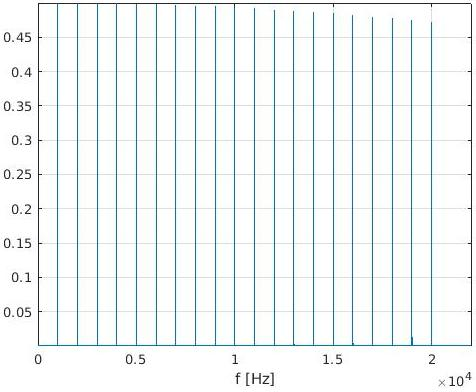
\includegraphics[scale=0.6]{images/Filter/input.jpg}}}%
	\qquad
	\subfloat[Filtered signal]{{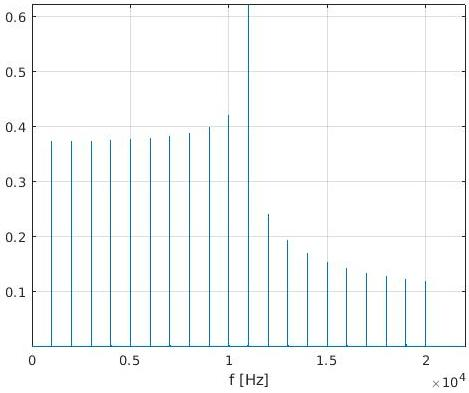
\includegraphics[scale=0.6]{images/Filter/response.jpg}}}%
	\caption{Spectrum (in magnitude) of the original and filtered signals}%
	\label{fig:filterMatlabTestbench}%
\end{figure}

As expected, the chosen filter has a low pass behavior with a cutoff frequency $F_c = 11.025 kHz$.

\subsection{Verilog implementation}

To evaluate the performance of the digital filter implemented in Verilog, a simulation is performed in Cadence. The testbench used for this purpose is to be found in \texttt{digital\_filter\_Testbench2}, and the corresponding schematic is provided in figure \ref{fig:filterTestbench}. it consists of a sum of sinus waveforms of 500Hz and 20 kHz respectively. For this simulation, an ideal ADC \texttt{adc\_ideal} has been additionally implemented, to convert the analog input signal to a digital one before filtering. The values for the different parameters are given in the table \ref{table:filterTestbench}. The order of the filter is deliberately small, in order to prevent a too important delay.\\
The obtained transient waveforms and spectrums are provided respectively in figures \ref{fig:filterCadenceTestbenchTransient} and \ref{fig:filterCadenceTestbenchSpectrum}. The ENOB, SINAD and SNR values are listed in the table \ref{table:filterValues}.
 

\begin{figure}[!h]
	\centering 
	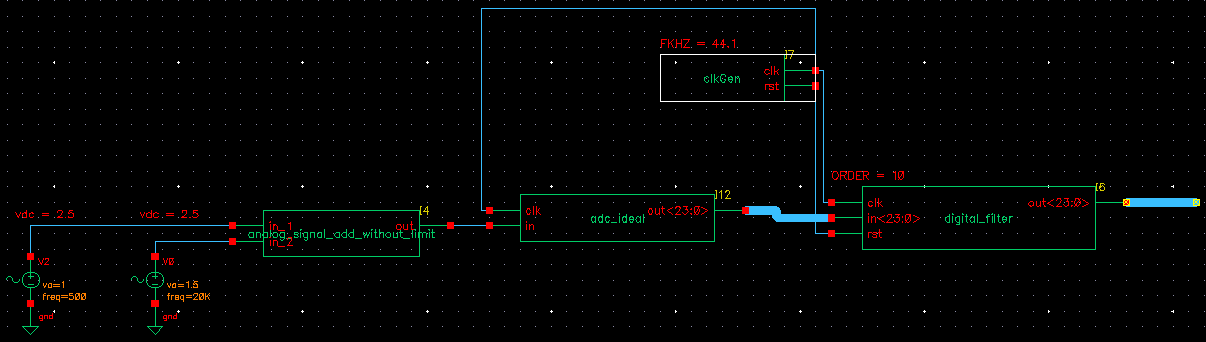
\includegraphics[scale=0.55]{images/Filter/testbench.png}
	\caption{Digital filter testbench}
	\label{fig:filterTestbench}
\end{figure} 

\begin{table}[!h]
	\centering
	\begin{tabular}{|l|r|}
		\hline
		Clock frequency (\texttt{FKHZ}) & 44.1 kHz \\
		\hline
		Filter order (\texttt{ORDER}) & 10 \\
		\hline
	\end{tabular}
	\caption{Filter testbench parameters}
	\label{table:filterTestbench}
\end{table}

\begin{figure}[!h]
	\centering 
	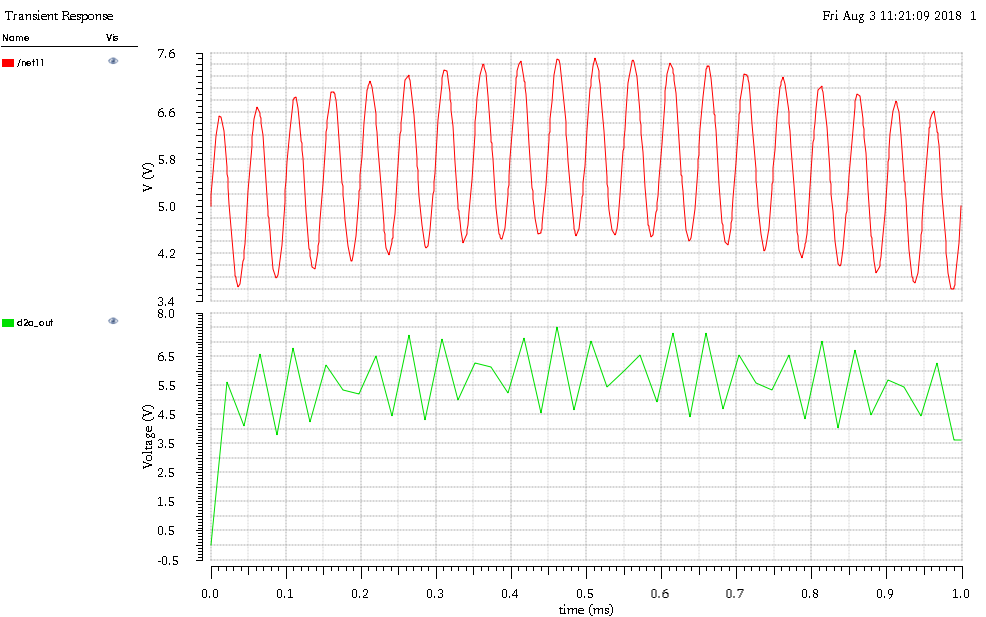
\includegraphics[scale=0.6]{images/Filter/signal.png}
	\caption{Transient simulation of the input (red) and filtered (green) signals}
	\label{fig:filterCadenceTestbenchTransient}
\end{figure} 

\begin{figure}[!h]
	\centering 
	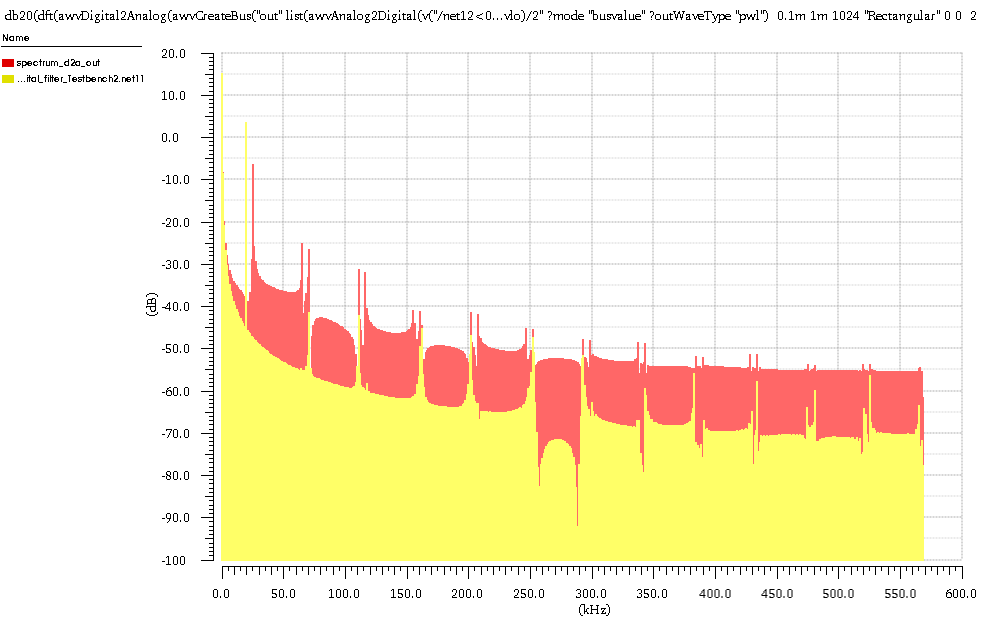
\includegraphics[scale=0.6]{images/Filter/spectrum.png}
	\caption{Spectrum of the input (yellow) and filtered (red) signals}
	\label{fig:filterCadenceTestbenchSpectrum}
\end{figure} 

\begin{table}[!h]
	\centering
	\begin{tabular}{|l|r|}
		\hline
		ENOB & -0.06092 bits \\
		\hline
		SINAD & 1.3963 dB \\
		\hline
		SNR & 1.3963 dB \\
		\hline
	\end{tabular}
	\caption{Filter statistics}
	\label{table:filterValues}
\end{table}

Surprisingly, the filtered signal contains more noise as the input signal. This may be due to the ADC which is working only at 44.1 kHz and may not capture the whole complexity of the input signal. Moreover, the relatively small order does not allow the filter to have a sharp cutoff of the higher frequencies.


\section{Synthesis}

The synthesis of the digital filter described above is performed using Synopsis Design Vision. The statistics obtained for different clock period are given in the table \ref{table:synthesisStats}.

\begin{table}[!h]
	\centering
	\begin{tabular}{|r|r|r|r|r|}
		\hline
		 \multirow{2}{*}{\textbf{Frequency}}
		 & \multirow{2}{*}{\textbf{Clock period [ns]}}
		 & \multirow{2}{*}{\textbf{Slack [ns]}} & \multicolumn{2}{c|}{\textbf{Area}} \\
		 \cline{4-5}
		 & & & \multicolumn{1}{c|}{\textbf{Cell}} & \multicolumn{1}{c|}{\textbf{Total}} \\
		\hline
		 1 GHz & 1 & - 1.78 & 31790.520257 & 54632.811374 \\
		 500 MHz & 2 & - 0.75 & 31881.240270 & 54705.954386 \\
		 \rowcolor{Blue}
		 333 MHz & 3 & 0.00 & 28362.240120 & 51198.672295 \\
		 250 MHz & 4 & 0.00 & 24488.640096 & 44641.649983 \\
		 200 MHz & 5 & 0.00 & 24275.520098 & 44453.918988 \\
		 \rowcolor{Green}
		 100 MHz & 10 & 0.00 & 23325.840074 & 41648.888715 \\
		 1 Hz & $10^{9}$ & ~$10^{9}$ & 23018.760042 & 47767.179669 \\
		\hline
	\end{tabular}
	\label{table:synthesisStats}
	\caption{Filter synthesis statistics}
\end{table} 

As shown in table \ref{table:synthesisStats}, the maximal clock frequency of the implemented filter is \textbf{333 MHz} (that is, a minimal clock period of \textbf{3 ns}). As expected, the required (cell and total) area is generally increasing with the frequency. Thus, the minimal total area is obtained for a frequency of \textbf{100 MHz}.
